\clearpage
\section*{Appendix: Supplementary Darknet results}
\addcontentsline{toc}{section}{Appendix: Supplementary Darknet results}

\begin{table}[H]
\centering
\begin{tabular}{lcc}
\toprule
Observable & Synthetic model & Empirical 2015 reference \\
\midrule
Mean degree & 99.31 & 99.31 \\
Average local clustering & 0.248 & 0.4 \\
Global clustering & 0.212 & 0.2 \\
Mean path length (LCC) & 2.4 & 2.5 \\
Diameter & 5 & 5 \\
Degree assortativity & $-0.154$ & -0.25 \\
\bottomrule
\end{tabular}
\caption{First synthetic realization versus the 2015 empirical reference.}
\label{tab:darknet-empirical-comparison}
\end{table}

\begin{figure}[H]
\centering
\begin{minipage}{.48\linewidth}\centering
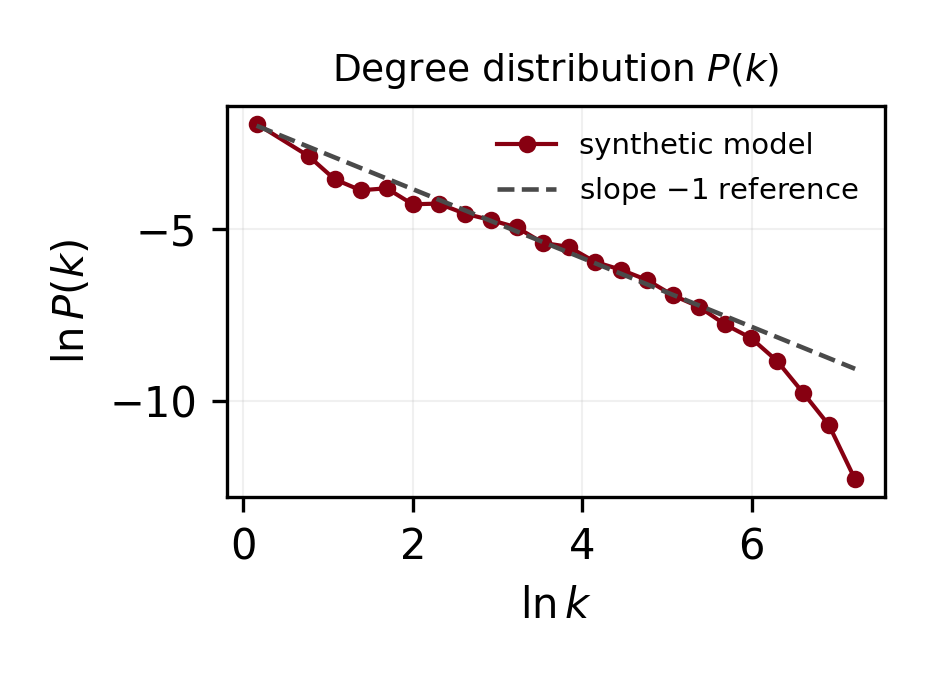
\includegraphics[width=.98\linewidth]{results/analysis_seed42/degree_distribution.png}
\end{minipage}\hfill
\begin{minipage}{.48\linewidth}\centering
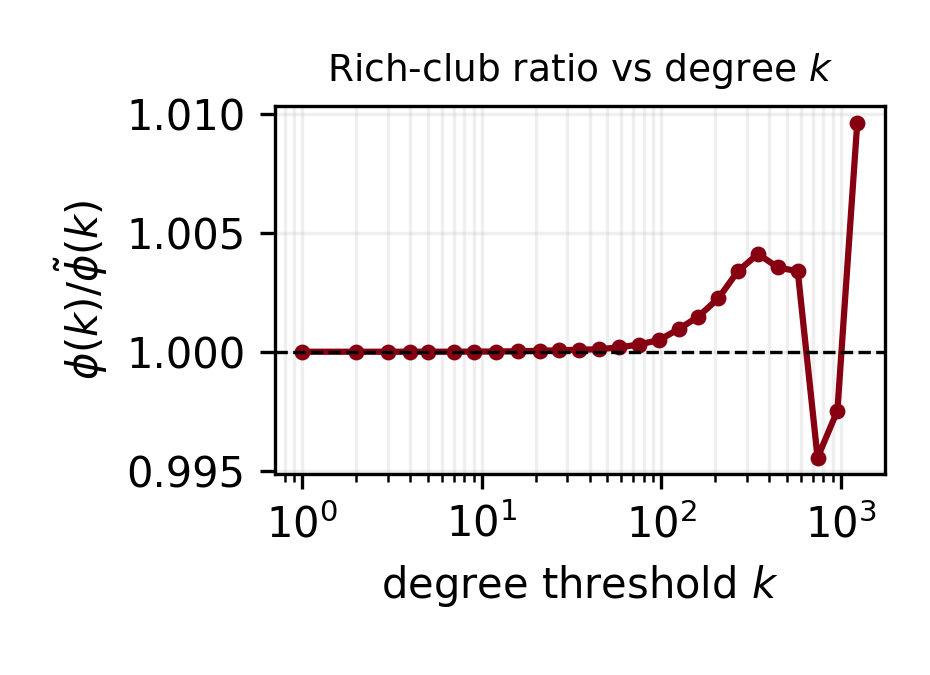
\includegraphics[width=.98\linewidth]{results/analysis_seed42/rich_club.png}
\end{minipage}
\medskip

\begin{minipage}{.48\linewidth}\centering
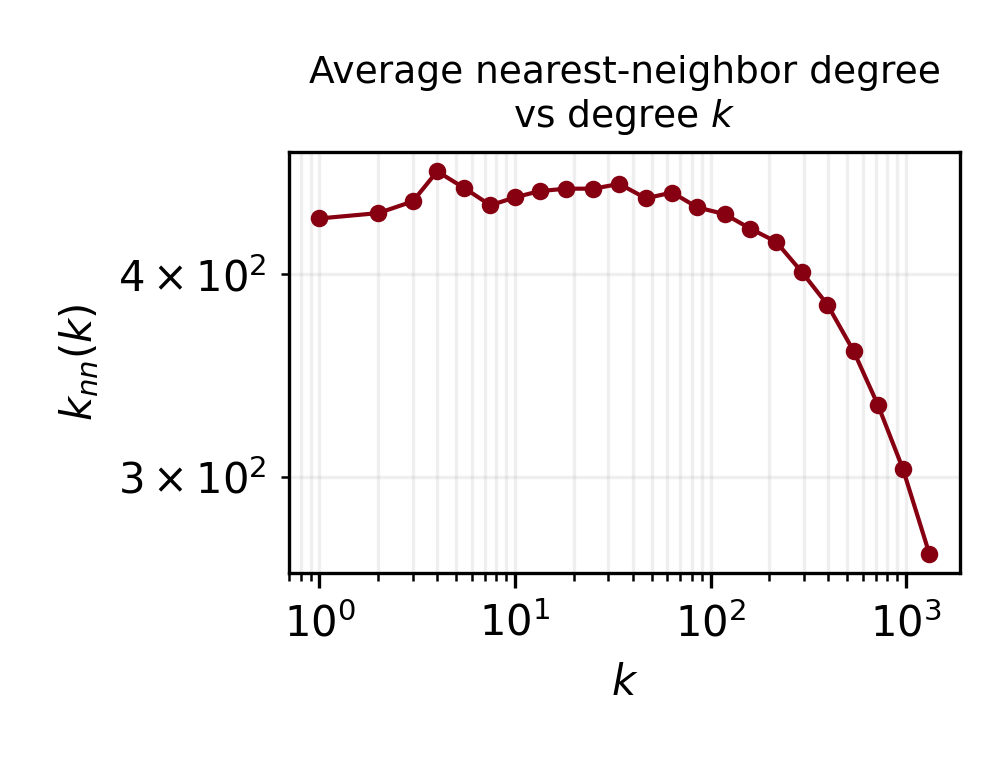
\includegraphics[width=.98\linewidth]{results/analysis_seed42/knn_by_degree.png}
\end{minipage}\hfill
\begin{minipage}{.48\linewidth}\centering
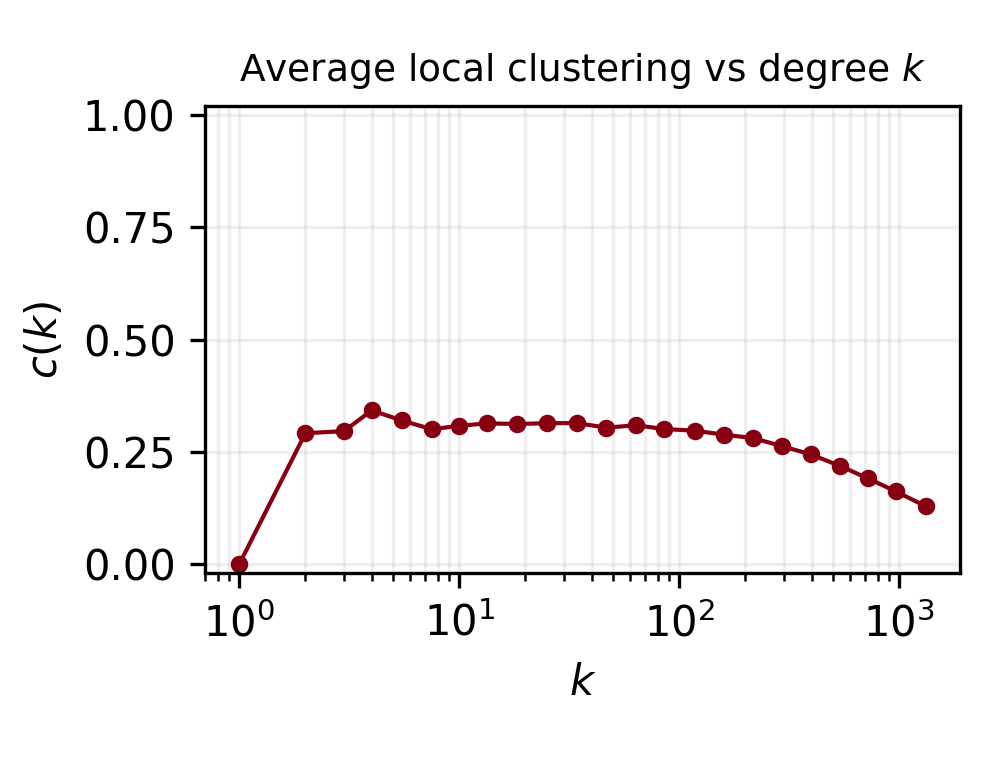
\includegraphics[width=.98\linewidth]{results/analysis_seed42/clustering_by_degree.png}
\end{minipage}
\caption{Structural and higher-order signatures of the synthetic model.}
\label{fig:darknet-structural-signatures}
\end{figure}
